\documentclass[a4paper,12pt]{article} % тип документа

% Поля страниц
\usepackage[left=2.5cm,right=2.5cm,
    top=2cm,bottom=2cm,bindingoffset=0cm]{geometry}
    
%Пакет дял таблиц   
\usepackage{multirow} 
    
%Отступ после заголовка    
\usepackage{indentfirst}


% Рисунки
\usepackage{floatrow,graphicx,calc}
\usepackage{wrapfig}

%%% Работа с картинками
\usepackage{graphicx}  % Для вставки рисунков
\graphicspath{{images/}{images2/}}  % папки с картинками
\setlength\fboxsep{3pt} % Отступ рамки \fbox{} от рисунка
\setlength\fboxrule{1pt} % Толщина линий рамки \fbox{}
\usepackage{wrapfig} % Обтекание рисунков и таблиц текстом

% Создаёем новый разделитель
\DeclareFloatSeparators{mysep}{\hspace{1cm}}

% Ссылки?
\usepackage{hyperref}
\usepackage[rgb]{xcolor}
\hypersetup{				% Гиперссылки
    colorlinks=true,       	% false: ссылки в рамках
	urlcolor=blue          % на URL
}


%  Русский язык
\usepackage[T2A]{fontenc}			% кодировка
\usepackage[utf8]{inputenc}			% кодировка исходного текста
\usepackage[english,russian]{babel}	% локализация и переносы

% Математика
\usepackage{amsmath,amsfonts,amssymb,amsthm,mathtools}

%%% Дополнительная работа с математикой
\usepackage{amsmath,amsfonts,amssymb,amsthm,mathtools} % AMS
\usepackage{icomma} % "Умная" запятая: $0,2$ $-$- число, $0, 2$ $-$- перечисление


% Что-то 
\usepackage{wasysym}


\begin{document}
\begin{center}
	\footnotesize{МОСКОВСКИЙ ФИЗИКО-ТЕХНИЧЕСКИЙ ИНСТИТУТ\\(НАЦИОНАЛЬНЫЙ 			ИССЛЕДОВАТЕЛЬСКИЙ УНИВЕРСИТЕТ)}\\
	\footnotesize{ФИЗТЕХ-ШКОЛА РАДИОТЕХНИКИ И КОМПЬЮТЕРНЫХ ТЕХНОЛОГИЙ\\}
	\hfill \break
	\hfill \break
	\hfill \break
	\hfill \break
	\hfill \break
	\hfill \break
\end{center}

\begin{center}   
    \hfill \break
	\hfill \break
	\hfill \break
	\hfill \break
	\hfill \break
	\hfill \break
	\hfill \break
	\hfill \break
	\hfill \break
	\hfill \break
	\hfill \break
	\large{Лабораторная работа № 4.7.3\\\large{\textbf{Поляризация}}}\\
	\hfill \break
        \hfill \break
	\hfill \break
	\hfill \break
	\hfill \break
	\hfill \break
	\hfill \break
	\hfill \break
	\hfill \break
	\hfill \break
	\hfill \break
	\begin{flushright}
		Климова Екатерина\\
		Группа Б01-108
	\end{flushright}
	\hfill \break
\end{center}
\hfill \break
\hfill \break
\begin{center}
	Долгопрудный, 2023 г.
\end{center}
\thispagestyle{empty}

\newpage
\hfill \break
\textbf{Цель работы:} ознакомление с методами получения и анализа поляризованного света.
\hfill \break
\hfill \break
\textbf{В работе используются:} оптическая скамья с осветителем; зеленый светофильтр; два поляроида; черное зеркало; полированная эбонитовая пластинка; стопа стеклянных пластинок; слюдяные пластинки разной толщины; пластинки в $1/4$ и $1/2$ длины волны; пластинка в одну длину волны для зеленого света (пластинка чуствительного оттенка).

\section{Аннотация}
\hfill \break В работе предлагается с помощью черного зеркала определить разрешенные направления поляроидов; определить характер поляризации света, прошедшего стопу и отраженного от нее под углом Брюстера; оценить угол Брюстера для эбонита; выделить пластинки $\lambda/4$ и $\lambda/2$; определить направления большей и меньшей скоростей для пластинки $\lambda/4$; исследовать интерференцию поляризованных лучей.

\section{Теоретические сведения}
\subsection{Определение направления разрешенной плоскости колебаний поляроида}
\hfill \break Определить направление разрешенных колебаний поляроида проще всего с помощью черного зеркала.

\hfill \break При падении света на отражающую поверхность под углом Брюстера свет в отраженном луче почти полностью поляризован, а вектор $\boldsymbol{E}$ параллелен отражающей поверхности (<<правило иголки>>). Луч света, прошедший поляроид и отразившийся от черного зеркала, имеет минимальную интенсивность при выполнении двух условий: во-первых, свет падает на отражающую поверхность под углом Брюстера и, во-вторых, в падающем пучке вектор $\boldsymbol{E}$ лежит в плоскости падения.

\hfill \break Вращая поляроид вокруг направления луча и черное зеркало вокруг оси, перпендикулярной лучу, методом последовательных приближений можно добиться минимальной яркости луча, отраженного от зеркала, и таким образом определить разрешенное направление поляроида.

\hfill \break Измеряя угол поворота зеркала (угол Брюстера), нетрудно определить коэффициент преломления материала, из которого изготовлено зеркало. Описанный метод часто используется для измерения коэффициента преломления непрозрачных диэлектриков.

\subsection{Получение эллиптически поляризованного света}
\hfill \break Элииптически поляризованный свет можно получить из линейно поляризованного с помощью двоякопреломляющих кристаллических пластинок.

\begin{wrapfigure}{r}{0.25\textwidth}
\begin{center}
    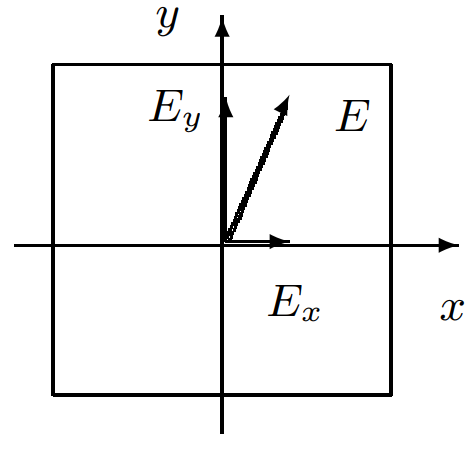
\includegraphics[width=1\textwidth]{4.7.3_1.png}
    \textbf{Рис. 1.} Разложение линейно поляризованного света по главным направлениям двоякопреломляющей пластинки
\end{center}
\end{wrapfigure}

\hfill \break Двоякопреломляющая пластинка имеет два взаимно перпендикулярных \textit{главных направления}, совпадающих с осями эллипсоида диэлектрической проницаемости. Волны, поляризованные вдоль главных направлений, распространяются в пластинке с разными скоростями, не изменяя характера своей поляризации. Эти волны называются \textit{главными}. Мы будем обозначать показатели преломления для главных волн через $n_{x}$ и $n_{y}$, где $x$ и $y$ $-$ главные направления кристаллической пластинки (рис. 1). 

\hfill \break Пусть на пластинку падает линейно поляризованная волна, электрический вектор которой ориентирован под некоторым углом $\alpha$ к оси $x$. Разложим вектор $\boldsymbol{E}$ на составляюшие $E_{x}$ и $E_{y}$. На входе пластинки $E_{x}$ и $E_{y}$ находятся в фазе. На выходе из-за разности скоростей между ними появляется разность хода $d(n_{x}-n_{y})$, при этом сдвиг фаз определяется соотношением:

\begin{equation}\label{ linkname }
\Delta \varphi = \frac{2\pi} {m} = kd(n_{x} - n_{y}),
\end{equation}

\hfill \break где $k$ $-$ волновое число (в пустоте), $d$ $-$ толщина кристаллической пластинки. При сложении двух взаимно перпендикулярных колебаний, обладающих некоторым сдвигом фаз, образуется колебание, поляризованное по эллипсу.

\hfill \break Рассмотрим практически важные частные случаи:

\begin{wrapfigure}{l}{0.25\textwidth}
\begin{center}
    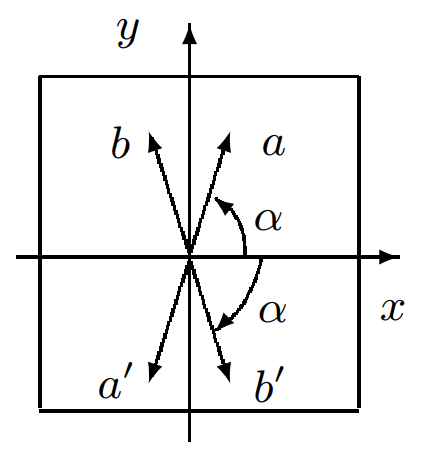
\includegraphics[width=1\textwidth]{4.7.3_2.png}
    \textbf{Рис. 2.} Поворот направления колебаний с помощью пластинки в $\lambda/2$
\end{center}
\end{wrapfigure}

\hfill \break а) Пластинка дает сдвиг фаз $2\pi$ (пластинка в длину волны $\lambda$). В результате сложения волн на выходе пластинки образуется линейно поляризованная волна с тем же направлением колебаний, что и в падающей волне.

\hfill \break б) Пластинка дает сдвиг фаз $\pi$ (пластинка в полдлины волны $\lambda$/2). На выходе пластинки снова образуется линейно поляризованная волна. Направление $bb'$ колебаний этой волны повернуто относительно направления $aa'$ колебаний падающей волны (рис. 2). Направление $bb'$ является зеркальным отображением направления $aa'$ относительно одного из главных направлений пластинки. Такую пластинку используют для поворота направления колебаний линейно поляризованного света.

\hfill \break в) Пластинка создает между колебаниями сдвиг фаз $\pi/2$ (пластинка в четверть длины волны). При сложении двух взаимно перпендикулярных колебаний, имеющих разность фаз $\pi/2$, образуется эллипс, главные оси которого совпадают с координатными осями $x$ и $y$. При равенстве амплитуд $E_{x}^{\text{max}} = E_{y}^{\text{max}}$ возникает круговая поляризация.

\hfill \break Следует отметить, что, говоря о пластинках $\lambda$, $\lambda/2$, $\lambda/4$ и т. д., всегда подразумевают какую-либо вполне определенную монохроматическую компоненту. Если на двоякопреломляющую пластинку падает не монохроматический свет, то на выходе из нее для разных спектральных компонент эллипсы поляризации будут различными.

\subsection{Анализ эллиптически поляризованного света}

\hfill \break Анализ эллиптически поляризованного света сводится к нахождению главных осей эллипса поляризации и к определению направления вращения электрического вектора.

\hfill \break Главные оси эллипса поляризации определяются с помощью анализатора по максимуму и минимуму интенсивности проходящего света. Направление вращения электрического вектора может быть найдено с помощью пластинки в четверть длины волны, для которой известно, какая из главных волн, $ E_x $ или $ E_y $, имеет б\'{o}льшую скорость распространения (и соответственно меньшее значение показателя преломления).

\hfill \break Выберем для определённости координатные оси $x$ и $y$ на пластинке так, чтобы $ nx < ny $. В этом случае главная волна $ E_x $ имеет большую скорость распространения. Поместим такую пластинку на пути эллиптически поляризованного света и совместим главные направления пластинки $ \lambda/4 $ с главными осями эллипса поляризации. На выходе из этой пластинки сдвиг фаз между $ E_x $ и $ E_y $ вместо $ \pi/2 $ станет равным нулю или $ \pi $. Свет окажется линейно поляризованным. Из двух возможных значений сдвига фаз, $0$ или $ \pi $, реализуется одно: то, которое соответствует имеющемуся в волне направлению вращения электрического вектора.

\hfill \break Рассмотрим, например, случай, когда электрический вектор в эллиптически поляризованной волне вращается против часовой стрелки, если смотреть навстречу лучу. В этом случае, очевидно, в волне, падающей на пластинку в $ \lambda/4 $, колебание $ E_y $ отстаёт по фазе на $ \pi/2 $ от колебания $ E_x $. При прохождении через пластинку разность фаз увеличивается до $ \pi $. Таким образом на выходе из пластинки возникают линейно поляризованные волны со сдвигом фаз $ \pi $. Сложение этих волн даёт плоскополяризованную волну, электрический вектор которой располагается во втором и четвёртом квадрантах координатной системы $x, \text{ } y$.

\hfill \break Рассуждая аналогичным образом, найдём, что при вращении электрического вектора по часовой стрелке направление колебаний в линейно поляризованной волне, выходящей из пластинки, располагается в первом и третьем квадрантах. Определяя направление колебаний на выходе из пластинки с помощью поляроида, можно, таким образом, определить характер эллиптической поляризации (вращение против или по часовой стрелке).

\subsection{Пластинка чувствительного оттенка}

\hfill \break Выше предполагалось известным, какому из двух главных направлений пластинки в четверть длины волны соответствует большая скорость распространения света. Установить это можно различными способами, например с помощью пластинки чувствительного оттенка (так называют пластинку в $ \lambda $ для зелёной спектральной компоненты, $ \lambda = 560 $ нм).

\hfill \break Пластинка имеет форму стрелы (рис. 3), вдоль оси которой расположено главное направление, соответствующее большей скорости распространения.

\hfill \break Если пластинка чувствительного оттенка помещена между скрещенными поляроидами и главные направления пластинки не параллельны направлениям разрешённых колебаний поляроидов, то при освещении белым светом пластинка кажется окрашенной в лилово-красный цвет. Это объясняется тем, что зелёная компонента линейно поляризованного света при прохождении пластинки не меняет поляризации и задерживается вторым поляроидом. Для красной и фиолетовой компонент пластинка создаёт сдвиг фаз, несколько отличный от $ 2\pi $. На выходе из пластинки красная и фиолетовая компоненты оказываются поэтому эллиптически поляризованными и частично проходят через второй поляроид. Таким образом, в известном смысле наблюдаемый в указанном опыте цвет пластинки дополнителен к зелёному.

\begin{wrapfigure}{l}{0.25\textwidth}
\begin{center}
    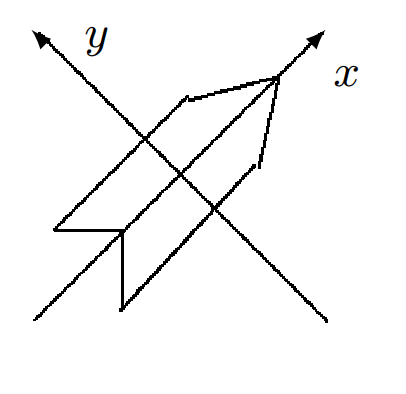
\includegraphics[width=1\textwidth]{4.7.3_3.png}
    \textbf{Рис. 3.} Пластинка чувствительного оттенка
\end{center}
\end{wrapfigure}

\hfill \break Если между скрещенными поляроидами поместить пластинку чувствительного оттенка ($ \lambda $) и пластинку в $ \lambda/4 $ так, чтобы их главные направления совпадали, цвет пластинки изменится. Если у пластинки чувствительного оттенка и пластинки в $ \lambda/4  $ совпадут главные направления, соответствующие большей скорости распространения, то разность хода между $ E_x $ и $ E_y $ для зелёного света составит уже $ 5\lambda/4 $. Это соответствует разности хода в $ \lambda $ для света с большей длиной волны, т. е. для <<более красного>> света. При освещении этих пластинок (напомним, что они расположены между скрещенными поляроидами) белым светом теперь погасится не зелёная, а красная часть спектра, и проходящий свет будет казаться зеленовато-голубым. Если же главные направления, соответствующие большей скорости распространения, у пластинки чувствительного оттенка и у пластинки в $ \lambda/4 $ окажутся перпендикулярными, то проходящий свет приобретет оранжево-желтую окраску (погасится фиолетово-голубая часть спектра).

\hfill \break Изменение цвета позволяет, таким образом, определить, какое из главных направлений пластинки в $ \lambda/4 $ соответствует большей скорости распространения.

\subsection{Интерференция поляризованных лучей}

\hfill \break Тонкие двоякопреломляющие пластинки, помещённые между поляроидами, кажутся окрашенными. Эта окраска может быть истолкована как результат интерференции поляризованных лучей. На рис. 4 представлена схема для случая скрещенных поляроидов.

\hfill \break Здесь $ p_1p'_1 $ $-$ разрешённое направление колебаний поляризатора (первого поляроида); $ x, \text{ } y $ $-$ координатная система, связанная с главными направлениями двоякопреломляющей пластинки; $ p_2p'_2 $ $-$ разрешённое направление колебаний анализатора (второго поляроида). Волны $ E_x  $ и $ E_y $ на выходе из пластинки когерентны, но не могут интерферировать, так как $ E_x \perp  E_y $. Волны $ E_1 $ и $ E_2 $ на выходе второго поляроида также являются когерентными и к тому же поляризованы в одной плоскости. Эти волны интерферируют между собой. Результат интерференции определяется зависящим от длины волны сдвигом фаз между $ E_1 $ и $ E_2 $. В результате интерференции поляризованных лучей пластинка, освещаемая белым светом, кажется окрашенной.

\begin{wrapfigure}{r}{0.25\textwidth}
\begin{center}
    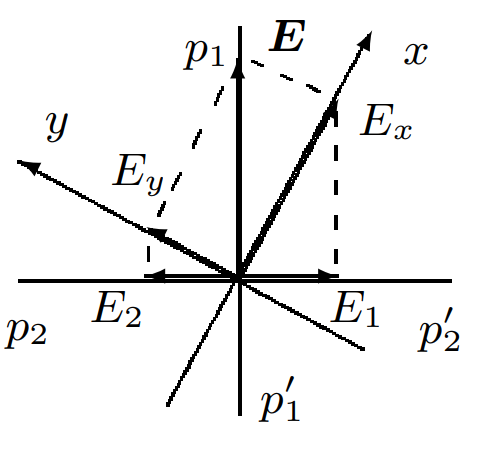
\includegraphics[width=1\textwidth]{4.7.3_4.png}
    \textbf{Рис. 4.} К объяснению интерференции поляризованных лучей
\end{center}
\end{wrapfigure}

\hfill \break Если поворачивать двоякопреломляющую пластинку, расположенную между скрещенными поляроидами, то соотношение амплитуд волн $ E_1 $ и $ E_2 $ и разность фаз между ними не изменяются. Это означает, что цвет пластинки при её поворотах не меняется, а меняется только интенсивность света. За один оборот пластинки интенсивность четыре раза обращается в нуль $-$ это происходит при совпадении главных направлений $ x $ и $ y $ с разрешёнными направлениями колебаний поляроидов.

\hfill \break Если же двоякопреломляющую пластинку оставить неподвижной, а второй поляроид повернуть так, чтобы разрешённые направления $ p_1p'_1 $ и $ p_2p'_2 $ совпали, то волны $ E_1 $ и $ E_2 $ приобретают дополнительный фазовый сдвиг на $ \pi $ для всех спектральных компонент; при этом их амплитуды изменятся так, что цвет пластинки изменится на дополнительный. 

\section{Экспериментальная установка}
\hfill \break На рис. 5, 6, 7, 8 представлены схемы экспериментальных установок, используемых в данной работе:	

\begin{center}
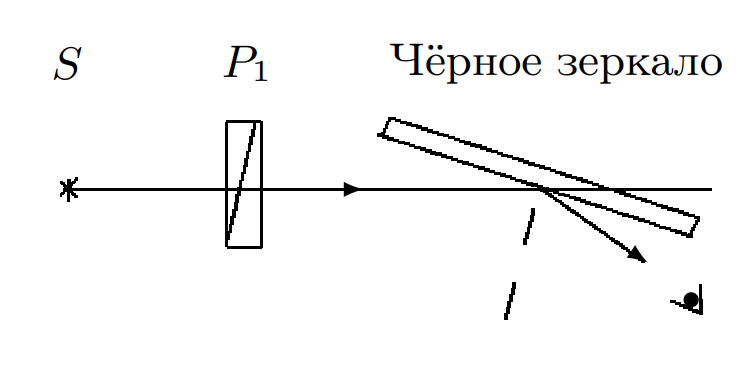
\includegraphics[width=0.45\textwidth]{4.7.3_5.png}\\
\textbf{Рис. 5.} Определение разрешенного направления поляроида \\
\end{center}

\begin{center}
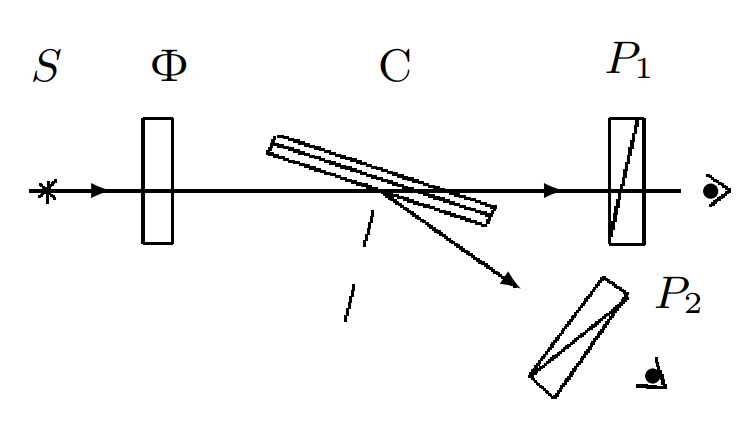
\includegraphics[width=0.45\textwidth]{4.7.3_6.png}\\
\textbf{Рис. 6.} Исследование стопы \\
\end{center}

\begin{center}
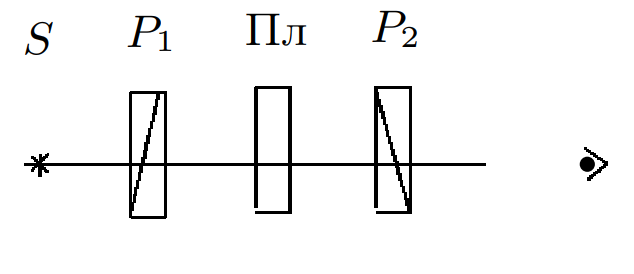
\includegraphics[width=0.45\textwidth]{4.7.3_7.png}\\
\textbf{Рис. 7.} Определение главных направлений в пластинках \\
\end{center}

\begin{center}
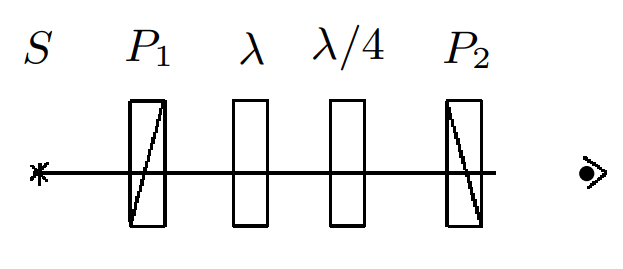
\includegraphics[width=0.45\textwidth]{4.7.3_8.png}\\
\textbf{Рис. 8.} Определение направлений большей и меньшей скоростей \\
\end{center}

\section{Ход работы}
\subsection{Определение разрешенных направлений поляроидов}
\hfill \break Разместим на оптической скамье осветитель $S$, поляроид $P_1$ и черное зеркало (рис. 5) так, чтобы плоскость падения была горизонтальна. Свет, отражённый от зеркала, рассматриваем сбоку, расположив глаз таким образом, чтобы вблизи оси вращения зеркала можно было увидеть изображение диафрагмы осветителя. Поворачивая поляроид вокруг направления луча, а черное зеркало вокруг вертикальной оси, методом последовательных приближений добьемся наименьшей яркости отраженного пятна. Определим разрешенное направление поляроида $-$ на лимбе $336^\circ$. 

\hfill \break Вместо черного зеркала поставим второй поляроид и определим его разрешенное направление, скрестив поляроиды: $40^\circ$.

\subsection{Определение угла Брюстера для эбонита}
\hfill \break Поставим на скамью вместо черного зеркала (рис. 5) эбонитовую пластину с круглой шкалой. Повернем эбонитовое зеркало вокруг вертикальной оси так, чтобы его плоскость была перпендикулярна лучу, и попытаемся совместить отражённое от эбонита пятно с отверстием осветителя. Установим направление разрешённых колебаний поляроида $P_1$ горизонтально и найдем угол поворота эбонита $\varphi_{\text{Б}}$, при котором интенсивность отражённого луча минимальна: его абсолютное значение равно $\varphi_{\text{Б}} = 304^\circ$.

\hfill \break Повторим измерения, добавив светофильтр Ф, и сравним результаты $-$ они получились одинаковыми.

\hfill \break По углу Брюстера рассчитаем показатель преломления эбонита:

$$
n_{\text{эксп}} = |\tg{\varphi_{\text{Б}}}| = |\tg{304^\circ}| \approx 1.48,
$$

\hfill \break притом что табличное значение показателя преломления эбонита $-$ $n_{\text{табл}} = 1.6$, что достаточно близко к экспериментальному.

\subsection{Исследование стопы}
\hfill \break Исследуем характер поляризации света в преломленном и отраженном от стопы лучах. Для этого поставим вместо эбонитового зеркала (рис. 5) стопу стеклянных пластинок под углом Брюстера. Осветим стопу неполяризованным светом и, рассматривая через поляроиды (рис. 6) отраженный от стопы и преломленный лучи, определим в них ориентацию вектора $\boldsymbol{E}$; затем определим характер поляризации света в преломленном луче. 

\hfill \break Наблюдая прошедший через стопу стеклянных пластинок луч света, убеждаемся, в том что плоскости
поляризации у отраженного и преломленного лучей взаимно перпендикулярны: угол на лимбе $P_1 = 328^\circ$, $P_2  = 235^\circ$. Преломленные лучи горизонтальные, отраженные $-$ вертикальные. Установили, что лучи имеют правый круговой тип поляризации.

\subsection{Определение главных направлений двоякопреломляющих пластин}
\hfill \break Определим главные направления двоякопреломляющих пластин. Для этого поставим кристаллическую пластинку между скрещенными поляроидами (рис. 7). Вращая пластинку вокруг направления луча и наблюдая за интенсивностью света, проходящего сквозь второй поляроид, определим, при каком условии главные направления пластинки совпадают с разрешенными направлениями поляроидов. Повторим опыт для второй пластинки. Результаты опытов занесем в таблицу;

\begin{center}
\begin{tabular}{|c|c|c|c|c|}\hline
$ $ & \multicolumn{2}{c|}{\text{Пластина 1}} &  \multicolumn{2}{c|}{\text{Пластина 2}} \\\hline
$ \text{min} $ & $ 62^\circ $ & $ 152^\circ $ & $ 18^\circ $ & $ 109^\circ $\\\hline
$ \text{max} $ & $ 106^\circ $ & $ 202^\circ $ & $ 70^\circ $ & $ 160^\circ $\\\hline
\end{tabular} \\
\hfill \break \textbf {Таблица 1.} Экстремумы интенсивности для пластин \\
\end{center}

\hfill \break Минимумы и максимумы интенсивности чередуются через $45^\circ$, главные плоскости пластин совпадают с разрешёнными направлениями поляроидов при максимальной интенсивности.

\subsection{Выделение пластин $\lambda/2$ и $\lambda/4$}
\hfill \break Для выделения пластин $\lambda/2$ и $\lambda/4$ добавим к схеме, изображенной на рис. 7, зеленый фильтр. Затем установим разрешенное направление первого поляроида горизонтально, а главные направления исследуемой пластинки $-$ под углом $45^\circ$ к горизонтали. С помощью второго поляроида установим, какую поляризацию имеет свет, прошедший пластинку: круговую или линейную с переходом в другой квадрант. 

\hfill \break Пластинка $\lambda/2$ не меняет характер поляризации, при её повороте \textit{меняется интенсивность}, а поляризация остаётся \textit{линейной}.

\hfill \break Проделаем то же со второй пластинкой: пластинка $\lambda/4$ создаёт сдвиг фаз $\pi/2$ между колебаниями $-$ эллиптическая поляризация. Эта пластинка \textit{не меняет интенсивность} при повороте.

\subsection{Определение направлений большей и меньшей скоростей в пластинке $\lambda/4$}
\hfill \break Определим <<быструю>> и <<медленную>> оси в пластинке $\lambda/4$. Поставим между скрещенными поляроидами пластинку чувствительного оттенка, имеющую вид стрелки (как на рис. 3), и убедимся, что эта пластинка не меняет поляризацию зеленого света в условиях предыдущего опыта. Световой вектор, ориентированный вдоль направления стрелки, проходит с большей скоростью, перпендикулярный $-$ с меньшей.

\hfill \break Уберем зелёный фильтр и поставим между скрещенными поляроидами пластинку $\lambda$ (стрелка под углом $45^\circ $ к разрешённым направлениям поляроидов). Глядя сквозь второй поляроид на стрелку, убедимся, что она имеет пурпурный цвет (зелёный свет задерживается вторым поляроидом, а красная и синяя компоненты проходят).

\hfill \break Добавим к схеме пластинку $\lambda/4$ (рис. 8), главные направления которой совпадают с главными направлениями пластины $\lambda$ и ориентированы под углом $45^\circ$ к разрешённым направлениям скрещенных поляроидов. При повороте рейтера со стрелкой на $180^\circ$ вокруг вертикальной оси цвет стрелки меняется от зелёно-голубого до оранжево-жёлтого. <<Быстрые>> оси совпадают, когда пластинка имеет зеленый цвет. 

\subsection{Интерференция поляризованных лучей}

\hfill \break Расположим между скрещенными поляроидами мозаичную слюдяную пластинку (рис. 9). Она собрана из 4-х узких полосок слюды, лежащих по сторонам квадрата (две полоски «толщиной» $\lambda/4$ и по одной $-$ $\lambda/2$ и $3\lambda/4$).

\begin{center}
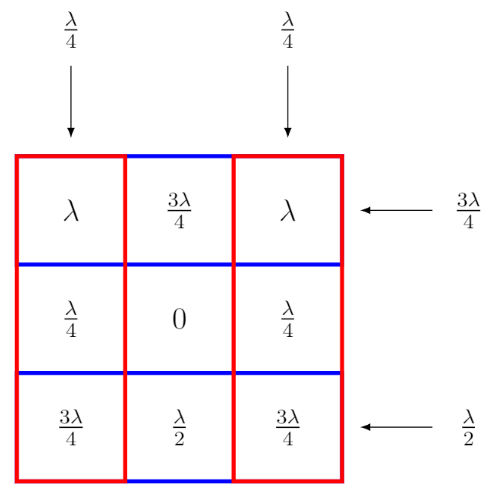
\includegraphics[width=0.55\textwidth]{4.7.3_11.png}\\
\textbf{Рис. 9.} Мозаичная слюдяная пластинка \\
\end{center}

\hfill \break В центральном квадратике слюды нет. Главные направления всех пластинок ориентированы параллельно сторонам квадрата. 

\hfill \break Вращая пластинку, будем наблюдать за изменениями в отдельном квадратике. Центральный квадратик всегда будет черным, что объясняется тем, что он не покрыт слюдой, а свет проходит через него и скрещенные поляроиды, поэтому интенсивность нулевая. При этом боковые квадратики изменяют как свой цвет, так и интенсивность с периодичностью $\pi/4$.

\hfill \break Не трогая пластинки, будем вращать второй поляроид. Теперь центральный квадратик изменяет интенсивность и цвет, так как в этом случае разрешенные направления поляроидов не являются скрещенными.

\subsection{Определение направления вращения светового вектора в эллиптически поляризованной волне}
\hfill \break Нарисуем эллипс поляризации для вектора $\boldsymbol{E}$, вышедшего из пластинки $\lambda$/4, и укажем на нём направления большей и меньшей скорости. На рисунке $x$ $-$ большая скорость, а $y$ $-$ меньшая. Рядом нарисуем две вышедших из пластинки синусоиды: $x(t)$ и $y(t)$ со сдвигом фаз в четверть периода. По рисунку направление вращения электрического вектора в эллиптически поляризованной волне против часовой стрелки.

\hfill \break \begin{center}
\begin{tabular}{cc}
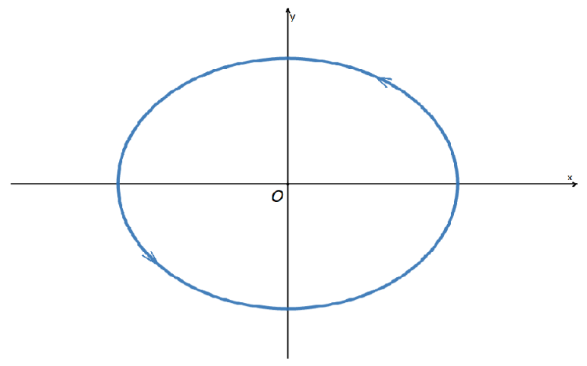
\includegraphics[width=0.5\textwidth]{4.7.3_9.png}&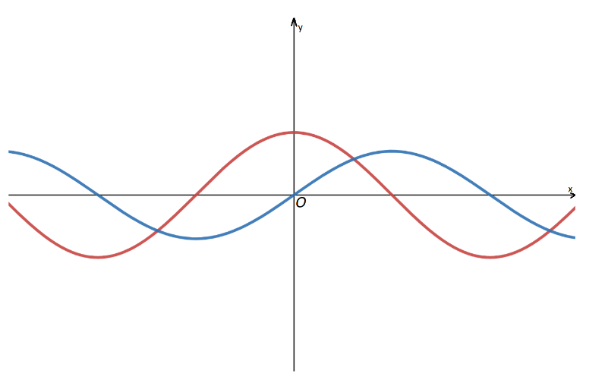
\includegraphics[width=0.5\textwidth]{4.7.3_10.png}\\
а) & б)\\
\end{tabular}
\hfill \break \textbf {Рис. 10.} Эллипс поляризации (а) и вышедшие из пластинки синусоиды (б) \\
\end{center}	
	
\hfill \break Снова поставим зелёный фильтр, а за ним между скрещенными поляроидами — пластинку $\lambda$/4 с соседней установки.
		
\hfill \break Получим эллиптически-поляризованный свет. Для этого установим разрешённое направление первого поляроида под углом $10^\circ$-$20^\circ$ к горизонтали так, чтобы вектор $\boldsymbol{E}$ падающего на пластинку света был расположен в первом квадранте. Установим разрешённое направление второго поляроида вертикально и, вращая пластинку, найдем минимальную интенсивность света, прошедшего второй поляроид. Вращая второй поляроид, убеждаемся, что свет поляризован эллиптически, а не линейно. Таким образом, был получен эллипс поляризации с вертикально ориентированной малой осью.

\hfill \break Для определения направления вращения светового вектора в эллипсе установим между поляроидами дополнительную пластинку $\lambda/4$ с известными направлениями «быстрой» и «медленной» осей, ориентированными по осям эллипса поляризации анализируемого света. В этом случае вектор $\boldsymbol{E}$ на выходе будет таким, как если бы свет прошёл две пластинки $\lambda/4$: свет на выходе из второй пластинки будет линейно поляризован. Если пластинки поодиночке дают эллипсы, вращающиеся в разные стороны, то, поставленные друг за другом, они скомпенсируют разность фаз, и вектор $\boldsymbol{E}$ на выходе останется в первом и третьем квадрантах. Если же световой вектор перешёл в смежные квадранты, значит, эллипсы вращаются в одну сторону.
		
\hfill \break По эксперименту получили, что после второго поляроида интенсивность света максимальна. Значит, две пластины усиливают друг друга, световой вектор перешёл в смежные квадранты, эллипсы вращаются в одну сторону. Таким образом, световой вектор в эллиптически поляризованной волне имеет направление вращения против часовой стрелки.

\section{Вывод}
\hfill \break В этой работе мы познакомились с методами получения поляризованного света и способами его анализа. Были определены разрешенные направления конкретных поляроидов, использованных в этой работе: $\alpha_1 = 336^\circ$ и $\alpha_2 = 40^\circ$. Был определен угол Брюстера для эбонита: $\varphi_{\text{Б}} = 304^\circ$, откуда был найден и показатель преломления: $n \approx 1.48$. Была исследована стопа Столетова, определены главные плоскости двоякопреломляющих пластин, а также направления большей и меньшей скоростей в пластинке в четверть длины волны. Мы пронаблюдали эллиптическую поляризацию и интерференцию поляризованных лучей. 

\end{document}